\documentclass{article}
% Se requieren los siguientes paquetes:
\usepackage{graphicx} % Requerido para insetar imágenes.
\usepackage{subcaption}%  Requerido para agrupar imagénes.
\usepackage{geometry}% Requerido para que existan simétricos espacios entre las imagénes agrupadas.
\usepackage{float} % Nos permite solucionar el problema en cuanto a carácteres y su relevancia.

\title{AGREGAR IMAGENES (INTERMEDIO)}
\author{Giuseppe Fuentes Moreno}
\date{September 2024}

\begin{document}

\maketitle

\section{Introduction}
a\\ % Las líneas "\\" expresan un salto de línea.
a\\
a\\
a\\
a
% Al introducir el comando "[H]", se superpone la imagén en el interior de la cádena de caracteres.
\begin{figure}[H]
    \centering
    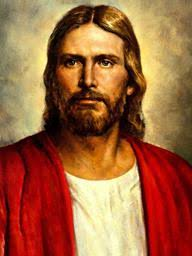
\includegraphics[width=0.3\linewidth]{descarga.jpeg}
    \caption{Jesucristo}
    \label{fig_1}
\end{figure}
b\\
b\\
\newpage %Con este comando, todo lo que se escribe depués se pone en la siguiente página.
Hola
% Para combinar dos imagénes cuadradas o rectángulares:
\begin{figure}
    \begin{subfigure}{0.49\textwidth}
        \centering
        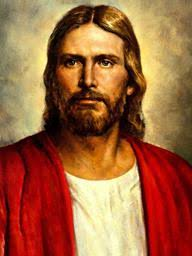
\includegraphics[width=\textwidth, heigth=10cm]{descarga.jpeg}
        \caption{Jesucristo 1 }
        \label{fig_2}
    \end{subfigure}
    \begin{subfigure}{0.49\textwidth}
        \centering
        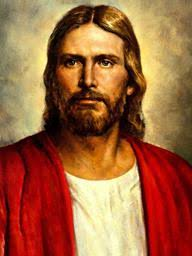
\includegraphics[width=\textwidth, heigth=10cm]{descarga.jpeg}
        \caption{Jesucristo 2 }
        \label{fig_3}
    \end{subfigure}
    \caption{Fotos de Jesús}
    \label{fig_4}
\end{figure}

%Para  añadir más figuras, añadimos los "\begin{subfigure}" que deseemos en el interior del comando "\begin{figure}".

%Si tenemos imagénes de mayor altura, reescribimos a nuestro gusto la altura de la imagén "heigth=4in" dónde "in" viene de pulgadas.

% Más info: "https://www.overleaf.com/learn/latex/Inserting_Images". 

\end{document}
